% Figure 2 — Training vs deployment, CLIP-style two panels.
% Aspect ratio ~2:1.  Same trained Theta in both panels — single-component
% invariance claim shown visually via a "frozen Theta" lock-pill bridging
% the two panels.
%
% Compile:  pdflatex figure2_training_deployment.tex

\documentclass[border=10pt, multi=tikzpicture]{standalone}

\usepackage[T1]{fontenc}
\usepackage{lmodern}
\usepackage{amsmath, amssymb}
\usepackage{tikz}
\usepackage{xcolor}

\usetikzlibrary{
  positioning,
  arrows.meta,
  shapes.geometric,
  shapes.symbols,
  calc,
  fit,
  backgrounds,
  decorations.pathmorphing,
}

\definecolor{cStatic} {HTML}{4C72B0}
\definecolor{cDynamic}{HTML}{55A868}
\definecolor{cFusion} {HTML}{8172B2}
\definecolor{cRUM}    {HTML}{C44E52}
\definecolor{cFrozen} {HTML}{7F7F7F}
\definecolor{cBPR}    {HTML}{B8732E}
\definecolor{cText}   {HTML}{1F2937}
\definecolor{cMuted}  {HTML}{6B7280}
\definecolor{cBorder} {HTML}{9CA3AF}

\begin{document}

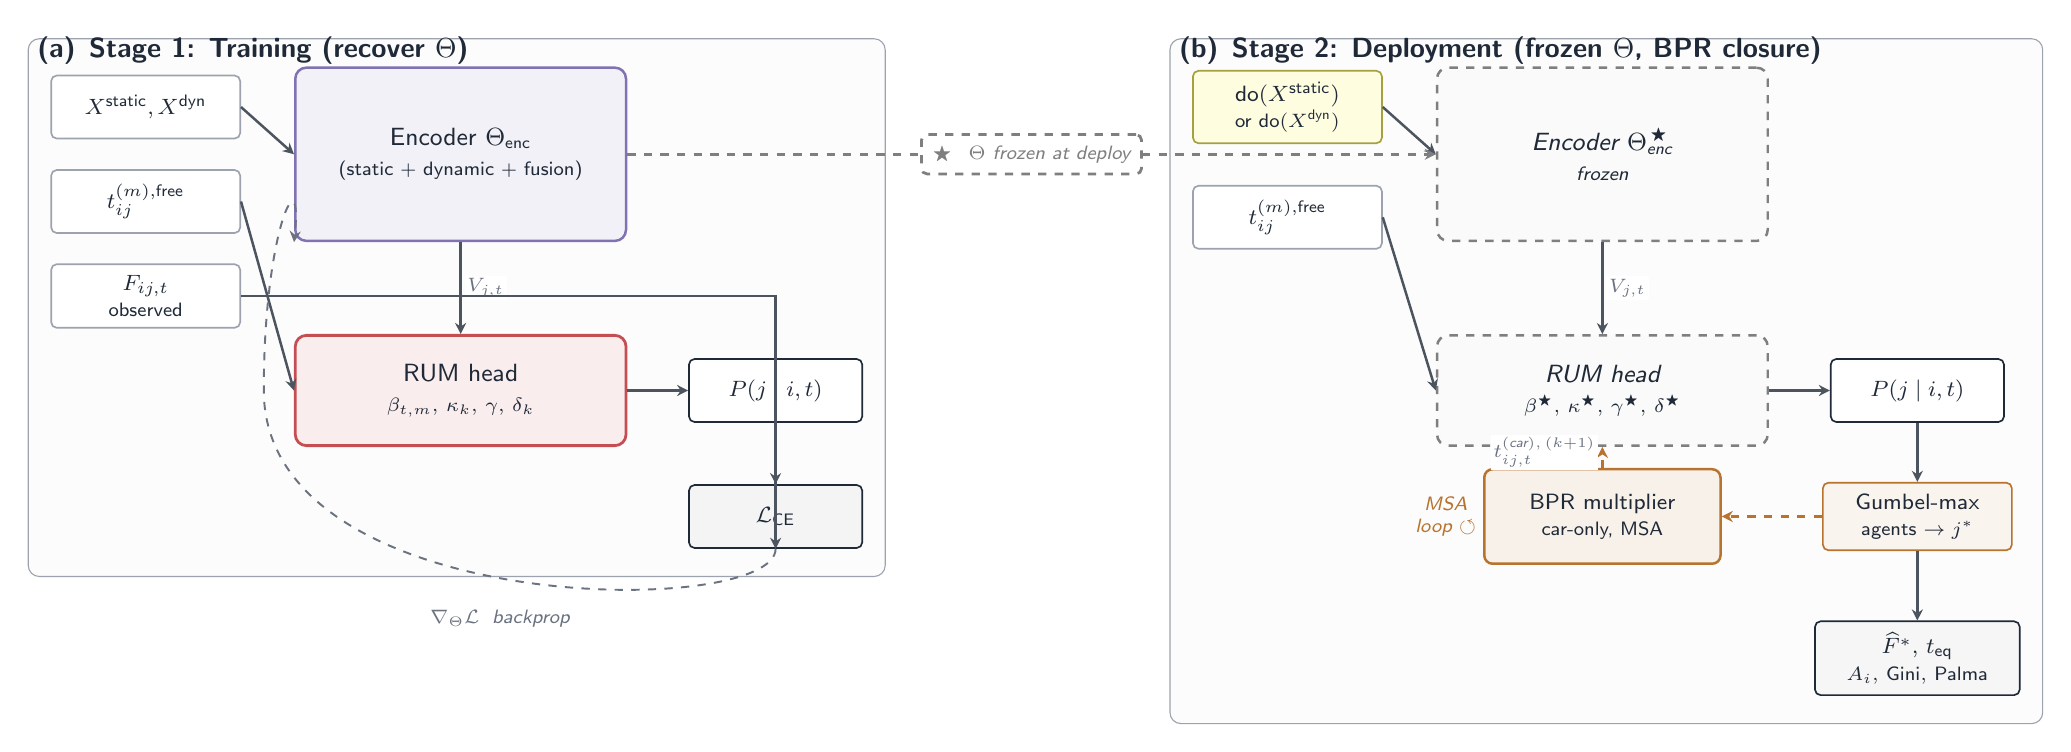
\begin{tikzpicture}[
  font=\sffamily\small,
  thick,
  >={Stealth[length=4pt, width=4pt]},
  every node/.style={align=center, text=cText},
  %
  panellabel/.style={font=\sffamily\bfseries, text=cText, anchor=north west},
  inputbox/.style={
    draw=cBorder, fill=white, line width=0.6pt,
    rounded corners=2pt, inner sep=4pt,
    minimum width=24mm, minimum height=8mm,
    font=\sffamily\footnotesize,
  },
  encbox trained/.style={
    draw=cFusion, fill=cFusion!10, line width=0.9pt,
    rounded corners=4pt, inner sep=6pt,
    minimum width=42mm, minimum height=22mm,
    font=\sffamily\small,
  },
  encbox frozen/.style={
    draw=cFrozen, fill=cFrozen!4, line width=0.9pt, dashed,
    rounded corners=4pt, inner sep=6pt,
    minimum width=42mm, minimum height=22mm,
    font=\sffamily\small\itshape,
  },
  rumbox trained/.style={
    draw=cRUM, fill=cRUM!10, line width=1.0pt,
    rounded corners=4pt, inner sep=6pt,
    minimum width=42mm, minimum height=14mm,
  },
  rumbox frozen/.style={
    draw=cFrozen, fill=cFrozen!4, line width=0.9pt, dashed,
    rounded corners=4pt, inner sep=6pt,
    minimum width=42mm, minimum height=14mm,
    font=\sffamily\small\itshape,
  },
  outbox/.style={
    draw=cText, fill=white, line width=0.6pt,
    rounded corners=2pt, inner sep=4pt,
    minimum width=22mm, minimum height=8mm,
    font=\sffamily\footnotesize,
  },
  bprbox/.style={
    draw=cBPR, fill=cBPR!10, line width=0.9pt,
    rounded corners=3pt, inner sep=5pt,
    minimum width=30mm, minimum height=12mm,
    font=\sffamily\footnotesize,
  },
  arr/.style={->, line width=0.8pt, draw=cText!75},
  arrFwd/.style={->, line width=0.9pt, draw=cText!80},
  arrBPR/.style={->, line width=0.9pt, draw=cBPR, dashed},
  arrlbl/.style={font=\sffamily\scriptsize\itshape, text=cMuted, fill=white,
                  inner sep=1pt, midway},
  panelframe/.style={draw=cBorder, fill=cText!1.5, rounded corners=4pt,
                      inner xsep=8pt, inner ysep=10pt},
]

% ════════════════════════════════════════════════════════════════════════
%  PANEL (a) — STAGE 1 TRAINING            absolute coords, X = 0..7 cm
% ════════════════════════════════════════════════════════════════════════

% inputs (left of panel a)
\node[inputbox] (a_in1)  at (0,  0)    {$X^{\text{static}}, X^{\text{dyn}}$};
\node[inputbox] (a_in2)  at (0, -1.2) {$t_{ij}^{(m), \text{free}}$};
\node[inputbox] (a_in3)  at (0, -2.4) {$F_{ij,t}$\\\scriptsize observed};

% encoder + RUM in middle of panel a
\node[encbox trained] (a_enc) at (4.0, -0.6)  {Encoder $\Theta_{\text{enc}}$\\\scriptsize{(static + dynamic + fusion)}};
\node[rumbox trained] (a_rum) at (4.0, -3.6)  {RUM head\\\scriptsize $\beta_{t,m},\,\kappa_k,\,\gamma,\,\delta_k$};

% output + loss on right of panel a
\node[outbox] (a_pjit) at (8.0, -3.6) {$P(j\mid i,t)$};
\node[outbox, fill=cText!5] (a_loss) at (8.0, -5.2) {$\mathcal{L}_{\text{CE}}$};

% arrows in panel (a)
\draw[arrFwd] (a_in1.east) -- (a_enc.west);
\draw[arrFwd] (a_in2.east) -- ($(a_rum.west)$);
\draw[arrFwd] (a_enc.south) -- node[arrlbl, right=1pt] {$V_{j,t}$} (a_rum.north);
\draw[arrFwd] (a_rum.east) -- (a_pjit.west);
\draw[arrFwd] (a_pjit.south) -- (a_loss.north);
\draw[arrFwd] (a_in3.east) -| (a_loss.south);

% backprop indicator: route AROUND boxes, going down-left then up-left
\draw[->, dashed, line width=0.7pt, draw=cMuted]
  (a_loss.south) .. controls (8.0, -6.5) and (1.5, -6.5) ..
  (1.5, -3.6) .. controls (1.5, -1.5) and (2.0, -0.6) .. (a_enc.south west);
\node[font=\sffamily\scriptsize\itshape, text=cMuted, fill=white, inner sep=1pt]
  at (4.5, -6.5) {$\nabla_\Theta \mathcal{L}$ \;backprop};

% panel (a) frame + label
\begin{pgfonlayer}{background}
  \node[panelframe, fit=(a_in1)(a_in3)(a_loss)(a_enc),
         label={[panellabel, yshift=4pt]north west:(a)\;\,Stage~1: Training (recover $\Theta$)}]
        (panelA) {};
\end{pgfonlayer}

% ════════════════════════════════════════════════════════════════════════
%  PANEL (b) — STAGE 2 DEPLOYMENT         absolute coords, X = 14..24 cm
% ════════════════════════════════════════════════════════════════════════

% inputs (left of panel b)
\node[inputbox, fill=yellow!12, draw=yellow!60!black]
                          (b_in1) at (14.5,  0)    {$\text{do}(X^{\text{static}})$\\\scriptsize{or }$\text{do}(X^{\text{dyn}})$};
\node[inputbox]           (b_in2) at (14.5, -1.4) {$t_{ij}^{(m), \text{free}}$};

% frozen encoder + RUM
\node[encbox frozen] (b_enc) at (18.5, -0.6)  {Encoder $\Theta_{\text{enc}}^{\,\bigstar}$\\\scriptsize{frozen}};
\node[rumbox frozen] (b_rum) at (18.5, -3.6)  {RUM head\\\scriptsize $\beta^{\bigstar},\,\kappa^{\bigstar},\,\gamma^{\bigstar},\,\delta^{\bigstar}$};

% choice + BPR + outputs on right
\node[outbox] (b_pjit) at (22.5, -3.6) {$P(j\mid i,t)$};

\node[outbox, fill=cBPR!8, draw=cBPR, minimum width=24mm]
                       (b_choice) at (22.5, -5.2) {Gumbel-max\\\scriptsize agents $\to j^{*}$};

\node[bprbox]          (b_bpr)    at (18.5, -5.2) {BPR multiplier\\\scriptsize car-only, MSA};

\node[outbox, fill=cText!4, draw=cText, minimum width=26mm]
                       (b_out)    at (22.5, -7.0) {$\widehat{F}^{*},\, t_{\text{eq}}$\\\scriptsize $A_i,\,\text{Gini},\,\text{Palma}$};

% arrows in panel (b)
\draw[arrFwd] (b_in1.east) -- (b_enc.west);
\draw[arrFwd] (b_in2.east) -- (b_rum.west);
\draw[arrFwd] (b_enc.south) -- node[arrlbl, right=1pt] {$V_{j,t}$} (b_rum.north);
\draw[arrFwd] (b_rum.east) -- (b_pjit.west);
\draw[arrFwd] (b_pjit.south) -- (b_choice.north);
\draw[arrFwd] (b_choice.south) -- (b_out.north);

% BPR feedback loop (orange dashed)
\draw[arrBPR] (b_choice.west) -- (b_bpr.east);
\draw[arrBPR] (b_bpr.north) -- node[arrlbl, near end, left=1pt]
              {$t_{ij,t}^{(\text{car}),\,(k+1)}$} (b_rum.south);
% MSA loop indicator
\node[font=\sffamily\scriptsize\itshape, text=cBPR, anchor=west]
   at (16.0, -5.2) {MSA\\loop $\circlearrowleft$};

% panel (b) frame + label
\begin{pgfonlayer}{background}
  \node[panelframe, fit=(b_in1)(b_in2)(b_enc)(b_rum)(b_bpr)(b_choice)(b_out),
         label={[panellabel, yshift=4pt]north west:(b)\;\,Stage~2: Deployment (frozen $\Theta$, BPR closure)}]
        (panelB) {};
\end{pgfonlayer}

% ════════════════════════════════════════════════════════════════════════
%  BRIDGING ELEMENT — "shared trained Theta" (lock pill)
% ════════════════════════════════════════════════════════════════════════
\draw[->, line width=1.0pt, draw=cFrozen, dashed]
  (a_enc.east) -- node[
    midway, fill=white, draw=cFrozen, rounded corners=2pt, inner sep=4pt,
    font=\sffamily\scriptsize\itshape, text=cFrozen,
  ] {$\bigstar$ \, $\Theta$ frozen at deploy} (b_enc.west);

\end{tikzpicture}

\end{document}
